\chapter{Evaluation}
\label{chap:evaluation}
In this chapter, our primary goal is to assess and examine the implementation of the \textbf{Scriburg} search engine while also drawing a comparison to the \textbf{ParseHub} solution. The evaluation process is organized into three main sections. Within Section \ref{sec:crawler-test}, we will conduct various experiments to assess the crawling process and discuss our findings and outcomes. In Section \ref{sec:indexer-test}, our focus will shift to evaluating the indexing procedure. Finally, in the last section, Section \ref{sec:ui-test}, we will explore user experience and the pros and cons of current user interface design.

\section{Testing Environment}
Demonstrating information about the testing machine used for the evaluation can provide enhanced clarity and facilitate meaningful comparisons to reproduce similar results.


\begin{table}[ht] 
\centering
{\footnotesize
\begin{tabular}{|P{3cm}|P{9.9cm}|}
 \hline
\textbf{Operating System} & Ubuntu 22.04.3 LTS \\ \hline
\textbf{CPU} & Intel(R) Core(TM) i7-10510U @ 1.80 GHz; 4 cores; 8 threads\\ \hline
\textbf{RAM} & 32 GB\\ \hline
\textbf{Machine} & Lenovo ThinkPad P15s Gen 1\\ 
\hline
    \end{tabular}
}
  \captionsetup{justification=centering,margin=2cm}
  \caption{The testing environment of the machine used in this evaluation.}
\end{table}

\section{Crawler}\label{sec:crawler-test}

Evaluating web crawlers can be challenging, but certain aspects can be discussed and reflected upon to provide a more comprehensive understanding of the crawler's performance and effectiveness.

{\renewcommand\labelitemi{}
\begin{itemize}
    \item \textbf{Coverage}: This can be accomplished by maintaining a list of the URLs of the targeted website and verifying whether the crawler successfully located and processed all of them. It is worth noting that precise measurement can be challenging because most websites do not disclose the total number of links they contain. Websites often undergo dynamic changes, resulting in some links being edited during the crawling process. Nevertheless, as previously mentioned, the evaluation metrics contribute to more comprehensively examining the crawler's performance and efficacy.

    \item \textbf{Scalability}: How manageable it is to scale the computing performance vertically and horizontally, allowing users to crawl more and bigger websites. 

    \item \textbf{Resilience}: Assessing the crawler's ability to navigate complex situations and handle errors, including its performance with inaccessible pages, broken links, slow networks, and dynamic content.

    \item \textbf{Politeness}:  The ability to respect the \texttt{robots.txt} rules and avoid getting blacklisted from the website's servers.

\end{itemize}

\subsection{Datasets} 
Evaluating a web crawler requires a more static website as a reliable reference point. Having a static website makes it easier to compare the content and the number of links. The \textbf{crawler-test}\footnote{A website suitable for crawler testing: \url{https://crawler-test.com/}} website is an excellent choice for this purpose due to its diverse content and links, containing a wide range of scenarios that a crawler might encounter. This website effectively employs \texttt{robots.txt} to guide the crawler, allowing for an assessment of its politeness. Moreover, it includes a section containing links yielding various HTTP request status codes, such as \textbf{4xx} and \textbf{5xx}, which is valuable for ensuring the crawler's robustness. Additionally, it incorporates multiple instances of page redirection, including scenarios like infinite redirection, which serves the dual purpose of evaluating the crawler's ability to avoid traps and enhancing its overall resilience.


To enhance the coverage and versatility of our crawler testing, we are considering three additional websites encompassing a broader range of use cases, ensuring that the crawler can effectively handle various HTML structures and more generic scenarios.
The first use case involves extracting product information from an e-commerce platform like \textbf{Douglas}\footnote{An e-commerce website: \url{https://www.douglas.de/}}. This website offers over 160,000 diverse products, making it an ideal candidate for testing different content types, including images.

The second website, \textbf{Times Higher Education}\footnote{Universities world ranking 2023: \url{https://www.timeshighereducation.com/world-university-rankings/2023/world-ranking}}, specializes in annually ranking universities. Since this website ranking is often updated yearly, it is a great candidate to test the coverage as we can count the number of universities easily.

The third website is \textbf{Stack Overflow}\footnote{Stack Overflow Python-related posts: \url{https://stackoverflow.com/questions/tagged/python}}. Given this website's extensive volume of questions, our focus will be specifically on Python-related questions. We will also limit the number of documents to be crawled.

\subsection{Experiments}
\subsection*{Crawler Test Base Evaluation}
As we mentioned, it is vital to test the crawler coverage, and the first website to test the crawler against is the \textit{crawler-test} website. 


\begin{table}[ht] 
\centering
{\footnotesize
\begin{tabular}{ |P{2.5cm}|P{8cm}|  }
 \hline
    \textbf{Seed URL\textsuperscript{*}} & \href{https://crawler-test.com/}{\texttt{https://crawler-test.com/}}\\ \hline
        \textbf{Inspectors\textsuperscript{*}} & \texttt{//*[contains(@class, 'large-12 columns')]}\\ \hline\hline
    \textbf{Allow Multi Elements} & False  \\ \hline
    \textbf{Max Pages} & 500\\ \hline
    \textbf{Threads} & 1\\ \hline
    \textbf{Max Depth} & 1 \\ \hline
    \textbf{Pagination} & None \\ \hline
    \textbf{Actions} & None\\ \hline
    \textbf{Max Docs} & 500\\ 
\hline
    \end{tabular}
}
  \captionsetup{justification=centering,margin=2cm}
  \caption{Crawler configuration for the crawler-test website}
  \label{table:crawler_test_config}
\end{table}

Table \ref{table:crawler_test_config} displays the crawler testing configurations used in the experiment. The Seed URL is set to the root path of the \textit{crawler-test}. The \textit{Allow Multi Elements} checkbox is disabled (set to False) because the objective is not to gather a list of documents; each page contains a single text field. The \textit{Max Pages} parameter is configured to a limit of 500, ensuring that the crawler does not exceed this number of pages. This figure can be adjusted based on the website's size to be crawled; for instance, smaller websites with around 50 pages may require a lower limit.
We have set the \textit{Max Depth} to 1 to enable easier coverage testing. This choice allows for easier comparison between the number of visited pages and the number of URLs discovered in the site's root path, which, upon simple page inspection, contains 415 links. Since the expected maximum number of pages is 415, the Max Docs parameter can be constrained to 500.
The inspectors are set to target the content of each page; thus, one inspector is only needed. No automated actions, such as scrolling or waiting, are necessary for this use case; therefore, they can be left. Any properties not explicitly mentioned can be left at their default settings.


\subsection*{Coverage Evaluation}
After creating a runner that runs, starts the crawling process, and is completed, the result of the crawler should be similar to the one shown in Table \ref{table:crawler_test_result}. Looking at the Links row, we can note that the crawler found 406 out of the expected 415 links. This is a coverage of 97.8\%. The other nine missing links can be excluded due to different reasons. Normalizing the links can result in duplicated links that can be skipped. 402 pages out of 406 found links are crawled correctly. The other four pages are categorized as \textit{Cross Site} links, meaning they do not belong to the \textit{Seed URL} hostname \texttt{crawler-test.com}. This is important to evaluate to ensure that the crawler stays focused, does not jump to sites out of the intended scope, and does not spend valuable resources. \textit{Already Visited} links is a counter that checks how many times the crawler found a link that has already been visited and skipped, in this case, 0. When no multithreading is used, and the \textit{Max Depth} is only set to 1, the \textit{Already Visited} is expected to be 0 because the duplicated links will be already excluded in the normalizing process before starting to crawl. 


\begin{table}[ht] 
\centering
{\footnotesize
\begin{tabular}{|P{1.5cm}|P{9.9cm}|}
 \hline
\textbf{Links} & 
\multicolumn{1}{c|}{\begin{tabular}{P{1.7cm}|P{1.7cm}|P{2.6cm}|P{2.5cm}|P{1.7cm}}
       \textbf{Collected}   & \textbf{Visited} & \textbf{Already Visited} & \textbf{Cross Site} &  \textbf{Excluded} \\
       406/415 & 402 & 0 & 4 & 1
\end{tabular}}

\\ 
\hline
\textbf{Time} & 
\multicolumn{1}{c|}{\begin{tabular}{ P{3.5cm}|P{3.5cm}|P{3.5cm}  }
       \textbf{Tot. Spent} & \textbf{Avg. Processing} & \textbf{Avg. Page Rendering}  \\
       671.19 s & 1.68 s & 0.697 s 
\end{tabular}}
\\
\hline
\textbf{Status Codes} & 
\multicolumn{1}{c|}{\begin{tabular}{P{2cm}|P{2cm}|P{2cm}|P{2cm}|P{2cm}}
              \textbf{1XX} & \textbf{2XX} & \textbf{3XX} & \textbf{4XX} & \textbf{5XX} \\
              2 & 328 & 4 & 52 & 15
\end{tabular}}
\\ 
\hline
\textbf{Docs \& Content} & 
\multicolumn{1}{c|}{\begin{tabular}{P{2.6cm}|P{2.6cm}|P{2.6cm}|P{2.6cm}}
       \textbf{Tot. Docs}   & \textbf{Duplicated Content} & \textbf{Avg. Docs Per Page} & \textbf{Avg. Page Size} \\
       255 & 24 & 1 & 1.6 MB
\end{tabular}}
\\ 
\hline
    \end{tabular}
}
  \captionsetup{justification=centering,margin=2cm}
  \caption{Completed crawler result of the crawler-test.com web site  }
    \label{table:crawler_test_result}
\end{table}


The \textit{Docs \& Content} section provides information regarding the collected and downloaded content. The \textit{Tot. Docs} metric indicates that 255 documents have been successfully downloaded. Twenty-five documents are duplicates and not saved in the database. This duplication is expected, as this testing site contains repetitive information designed to verify the functionality of this feature.
The \textit{Avg. Docs Per Page} value is 1, indicating that the site typically presents one document per page. 

\subsection*{Performance Evaluation}
Evaluating the performance of a web crawler is challenging as it depends on different aspects, such as the page's size and how fast the page loads. Moreover, if the site uses pagination, this can add extra waiting time to render the rest of the content. Furthermore, adding additional machines to enhance performance while not overburdening the server with excessive requests is possible, presenting a challenging balance between achieving excellent performance and maintaining proper politeness. However, some valuable matrices can be helpful to give a good insight like those shown in the Time row in Table \ref{table:crawler_test_result}. The total time spent to crawl \textbf{402 pages} took approximately \textbf{11 minutes}. To give a better perspective, the enterprise solution \textbf{ParseHub} \footnote{ParseHub plans: \url{https://www.parsehub.com/pricing}} the free plan (without IP Rotation\footnote{IP rotation is the practice of periodically changing the public IP address used by a device or server to improve security, avoid detection, or access geographically restricted content.}), can crawl \textbf{200 pages} in \textbf{40 minutes}, and the Standard expensive plan (with IP Rotation) that costs \$189 can crawl 200 pages in 10 minutes. This means crawling the \textbf{402 pages} inside the \textit{crawler-test} will take \textbf{20 minutes}. Comparing the crawler with the ParseHub, it is two times faster than the standard plan and eight times faster than the free plan. Note that in this evaluation, the performance can be increased by using more threads or nodes to distribute the loads, which we will evaluate. 


While some crawlers can achieve crawling rates of up to \textbf{300 pages/second} \cite{shkapenyuk2002design}, this comparison is not applicable. Crawling 300 pages from the same domain, as we are doing, is more challenging than simply crawling 300 different pages from 300 different websites. Distributing 300 HTTP requests evenly across these 300 websites is acceptable and does not result in a Denial of Service (DoS) issue because each domain receives only one request per second. However, in the context of Scriburg, users aim to target a specific set of websites, which could include just one website. If we send 300 requests to the same website, it could overload and crash the site.

\subsection*{Rendering Dynamic Content Evaluation}
Improving the average page rendering time (\textbf{0.679 seconds}) in Table \ref{table:crawler_test_result} is achievable by avoiding using rendering engines like Selenium. Processing a simple HTTP request is often quicker than rendering the entire page and waiting for the page to finish loading. However, it is essential to note that the rendering step is crucial in handling dynamic content. For instance, consider the dynamically inserted text, indicated by the link \footnote{Rendering test: \url{https://crawler-test.com/javascript/dynamically-inserted-text}}. This link is a straightforward example to illustrate the significance of the rendering process for web crawlers.

Using a simple \texttt{wget}\footnote{wget is a command-line utility for retrieving files from the internet using HTTP, HTTPS, FTP, and FTPS protocols, primarily used in Unix-like operating systems.} command in Linux, one can download the content shown in \ref{lst:no_rendering}. This content reveals that the HTML tags, \texttt{h1} and \texttt{p}, lack the inner text the crawler can collect as a document. Although a JavaScript code is designed to replace the \texttt{innerHTML} for each tag with text, without a rendering engine, the JavaScript logic remains unexecuted. Consequently, gathering the inner text of these tags becomes an impossibility. On the other hand, \ref{lst:rendered} shows the same page content after rendering where both tags are updated, and both contain the right content that the crawler can see and download.

\lstset{language=HTML}
{\footnotesize
\begin{lstlisting}[frame=single, caption={The dynamically-inserted-text link content before rendering},captionpos=b, label={lst:no_rendering.}]
<body>
  <h1 id="h1"></h1> 
  <p id="par"></p>
  <script>
    document.getElementById("h1").innerHTML = 'Some random text';
    document.getElementById("par").innerHTML = 'Some long content ...'; 
  </script>
</body>
\end{lstlisting}}


While this is a simplified example, it is easy to visualize more complicated websites employing advanced JavaScript frameworks and libraries for client-side rendering. This complexity increases the rendering time due to the execution of all JavaScript logic and the subsequent updating of the HTML DOM. Given that the crawler's objective is to locate and collect all HTML content, it is essential to discover all the HTML content. 


\lstset{language=HTML}
{\footnotesize
\begin{lstlisting}[frame=single, caption={The dynamically-inserted-text link content after rendering.},captionpos=b, label={lst:rendered}]
<body>
  <h1 id="h1">
    'Some random text'
  </h1> 
  <p id="par">
    'Some long content ...'
  </p>
  <script>
    document.getElementById("h1").innerHTML = 'Some random text';
    document.getElementById("par").innerHTML = 'Some long content ...'; 
  </script>
</body>
\end{lstlisting}}

\subsection*{Robustness and Politeness Evaluation}
The \textit{Status Codes} metric captured in Table \ref{table:crawler_test_result} reveals the variety of distinct status codes encountered while crawling. Given that this website serves as a testing ground for various scenarios, it naturally exhibits a range of status codes. Evaluating the crawler's resilience across these diverse cases is vital for enhancing its stability. The crawler should remain operational even when encountering a status code other than \textbf{2xx}.
In the specific test case, it is worth noting that the crawler confronted 66 different status codes without terminating and completed the crawling operation. This outcome encompasses status codes from the \textbf{1xx}, \textbf{2xx}, \textbf{3xx}, \textbf{4xx}, and \textbf{5xx} ranges. In contrast, testing ParseHub to crawl the same links from the crawler-test website hangs at some links. One of the links that ParseHub stopped crawling and hanging was the redirect link\footnote{Redirect page test: \url{https://crawler-test.com/redirects/redirect_target}}.

The \textit{Tot. Errors} metric accounts for various Selenium exceptions\footnote{Selenium exceptions:  \url{https://www.selenium.dev/selenium/docs/api/py/common/selenium.common.exceptions.html}} that may arise during the crawling process. As mentioned, many errors are expected since this is a testing site with different edge cases, and not terminating under those conditions is a good indication.

The presence of the \texttt{robots.txt} flag covers the commitment to polite crawling behavior. The flag is set to True when this file is located and successfully downloaded. It is essential to emphasize the importance of respectful crawling and commitment to the \texttt{robots.txt} file protocol. For monitoring purposes, the \textit{Excluded} links in Table \ref{table:crawler_test_result} record the count of links disallowed from being crawled. In this specific test case, there was only a single disallowed link. 

\subsection*{Changing Crawler Depth}

Up to this point, our evaluation of the crawler has been limited to a single page to assess its simplicity and test its coverage. However, the crawler's functionality should extend beyond merely identifying links; it should also be able to navigate between them and continuously gather the target documents. The next step is to evaluate if the crawler jumps between pages and can increase the coverage. To evaluate this, we will change the \textit{Max Depth} from 1 to 10. This will allow the crawler to jump up to 10 levels deeper, collecting more links and documents. Table \ref{table:crawler_test_config_depth_10} shows the configurations used for this test case. In practice, determining the precise depth can be challenging. In many cases, this number can be aligned with the pagination structure on the website, as the goal is to navigate through all pagination pages until they are completed. If the exact number is unknown, an approximate value can be assigned.

\begin{table}[ht]
\centering
{\footnotesize
\begin{tabular}{ |P{2.5cm}|P{8cm}|  }
 \hline
\textbf{Seed URL\textsuperscript{*}} & \href{https://crawler-test.com/}{\texttt{https://crawler-test.com/}}\T\B 
\\ 
\hline
\textbf{Inspectors\textsuperscript{*}} & \texttt{//*[contains(@class, 'large-12 columns')]}\T\B 
\\ \hline\hline
\textbf{Allow Multi Elements} & False \T\B 
\\ 
\hline
\textbf{Max Pages} & 1000\T\B 
\\ 
\hline
\textbf{Threads} & 1\T\B 
\\ 
\hline
\textbf{Max Depth} & 10\T\B 
\\ 
\hline
\textbf{Pagination} & None\T\B 
\\ 
\hline
\textbf{Actions} & None\T\B 
\\  
\hline
\textbf{Max Docs} & 1000\T\B 
\\ 
\hline
    \end{tabular}
}
  \captionsetup{justification=centering,margin=2cm}
  \caption{Crawler configuration for the crawler-test website, increasing the depth to 10}
    \label{table:crawler_test_config_depth_10}
\end{table}

Unfortunately, knowing exactly how many links the entire crawler-test site contains is challenging. However, since we have evaluated how the crawler behaves when the \textit{Max Depth} equals one to test only the home page, we can have some degree of assurance on the rest of the results on the rest of the pages. The Table \ref{table:crawler_test_result_depth_10} shows 895 links have been found. This number was expected to increase compared to the first evaluation when the \textit{Max Depth} equals one where the collected links were 406. 

Given the increase in depth to 10, we anticipate more documents being collected. We would raise the maximum page limit and the maximum number of collected documents to allow the crawler to crawl more pages. One vital difference between setting the \textit{Max Depth} and \textit{Max Pages} is that if one single page contains 1000 links, and the \textit{Max Depth} is set to 1, then all the 1000 pages will be visited because all are living in the first level of crawling (home page with level equals to one) so limited by the depth only will not work. This is the reason for adding the \textit{Max Page} as a termination condition.
\begin{table}[ht] 
\centering
{\footnotesize
\begin{tabular}{|P{1.5cm}|P{9.9cm}|}
 \hline 
\textbf{Links} & 
\multicolumn{1}{c|}{\begin{tabular}{P{1.7cm}|P{1.7cm}|P{2.6cm}|P{2.5cm}|P{1.7cm}}
       \textbf{Collected}   & \textbf{Visited} & \textbf{Already Visited} & \textbf{Cross Site} &  \textbf{Excluded} \\
       895 & 697 & 0 & 198 & 1
\end{tabular}}
\\ 
\hline
\textbf{Time} & 
\multicolumn{1}{c|}{\begin{tabular}{ P{3.5cm}|P{3.5cm}|P{3.5cm}  }
       \textbf{Tot. Spent} & \textbf{Avg. Processing} & \textbf{Avg. Page Rendering}  \\
       760.84 s & 3.26 s & 1.03 s 
\end{tabular}}
\\
\hline
\textbf{Status Codes} &      
\multicolumn{1}{c|}{\begin{tabular}{P{2cm}|P{2cm}|P{2cm}|P{2cm}|P{2cm}}
              \textbf{1XX} & \textbf{2XX} & \textbf{3XX} & \textbf{4XX} & \textbf{5XX} \\
              2 & 292 & 4 & 47 & 15
\end{tabular}}

\\ 
\hline
\textbf{Docs \& Content} & 
\multicolumn{1}{c|}{\begin{tabular}{P{2.6cm}|P{2.6cm}|P{2.6cm}|P{2.6cm}}
       \textbf{Tot. Docs}   & \textbf{Duplicated Content} & \textbf{Avg. Docs Per Page} & \textbf{Avg. Page Size} \\
       375 & 667 & 1 & 1.6 MB
\end{tabular}}
\\ 
\hline
    \end{tabular}
}
  \captionsetup{justification=centering,margin=2cm}
  \caption{Completed crawler result of the crawler-test.com
web site when the depth is 10.}
      \label{table:crawler_test_result_depth_10}
\end{table}

When comparing the increased depth test of the base crawler to the base one in the previous test, one notable metric is the significant increase in \textit{Cross Site} links from 4 to 198. Typically, this suggests that the crawler is attempting to navigate beyond the originating website specified in the seed URL. When this number rises, it often indicates a need to adjust and refine the crawler settings. However, in the case of this test website, such an increase is expected and considered normal. This is because the website intentionally includes various tests designed to redirect the crawler to external websites. While search engines like Google benefit from crawling across different domains to index multiple websites, our specific crawler primarily focuses on a single website, as this aligns with the user's typical interest.

\subsection*{Multithreading Evaluation}

It is crucial to assess the scalability of the crawler, primarily since it uses a unique links-sharing multithreading pool. We must thoroughly test it. We will use the same configurations detailed in Table \ref{table:crawler_test_config_depth_10} but adjust the threads parameter and monitor the overall time spent. The results are presented in Figure \ref{fig:threads-table}, illustrating the outcomes of eight different runs using identical crawler settings while varying the number of threads.

When we switch from \textbf{one} thread to \textbf{two}, we observe a reduction in time from \textbf{722 seconds} to \textbf{595 seconds}, representing a $\textbf{17.6\%}$ improvement, and increasing the threads to \textbf{four} results in a time of \textbf{438 seconds}, which is a $\textbf{39.33\%}$ improvement compared to using just \textbf{one} thread. However, further increasing the threads to \textbf{six} or \textbf{eight} does not yield any additional performance enhancements in comparison to using \textbf{four} threads. This is primarily because all threads communicate to share unvisited links and avoid revisiting links already processed by other threads. Consequently, as the number of threads increases, the communication between threads and the resources sharing (database, logs, and buffers) overhead escalates.
Users must fine-tune this parameter until they find the optimal setting, which appears to be \textbf{four} threads in the tested local environment.

\begin{figure}[H]	
     \centering
     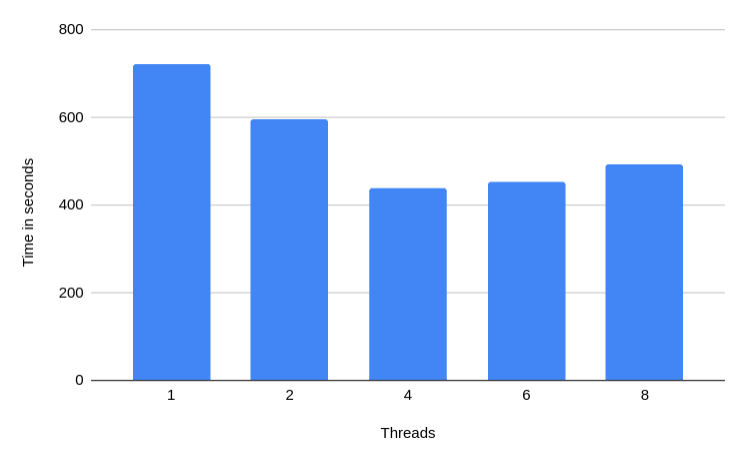
\includegraphics[width=10cm]{figures/threads-table.png}
     \captionsetup{justification=centering,margin=2cm}
     \caption{Multithreading performance comparison. }
     \label{fig:threads-table}
\end{figure}


Another vital step in evaluating the effectiveness of multithreading is examining the distribution of shared links among threads. This is crucial to prevent one thread from overburdening while others remain inactive, which would be inefficient, especially when using cloud services like AWS, where resources come at a cost. We will evaluate using the same configurations from Table \ref{table:crawler_test_config_depth_10}, employing four threads and rerunning the same crawler four times.

To test the workload of each thread, we rerun a crawler with four threads four times and calculated each thread and how many documents each has collected. Then, the average of those four runs is also recorded. Figure \ref{fig:threads-share} displays the results of four runs, with each run showcasing the distribution of crawled documents among each thread. 

\begin{figure}[H]	
     \centering
     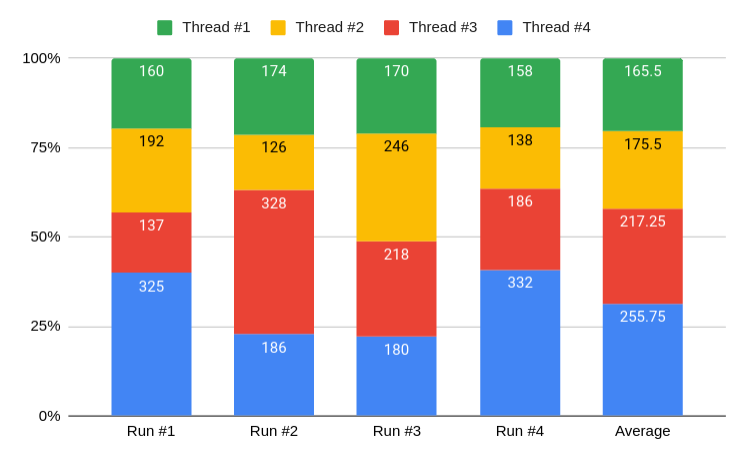
\includegraphics[width=10cm]{figures/threads_share.png}
  \captionsetup{justification=centering,margin=1cm}

     \caption{The workload distribution among four threads in four different runners. The chart shows each thread how many documents it has collected and the percentage.}
     \label{fig:threads-share}
\end{figure}

While the ideal scenario would involve each thread downloading \textbf{25\%} of the collected links, the chart shows otherwise. Looking at the \textit{Average} column, we can note that thread number \textbf{$4$} crawls more than \textbf{25\%}, while thread number \textbf{1} crawls less, which is expected because as long as one thread contains less than five links, it will keep crawling those links, and the other threads will remain idle. Only when the thread contains more than five links in the queue will it share those links with one other thread, and the others will remain idle. 

For example, if a website contains only ten links, then only two threads will be needed, where each will process five links, and the other two threads will stay idle. We do not split all ten links among the threads equally because we want to reduce the thread's communication and resource-sharing overhead, and we only use a thread when needed. 

Although each thread was not precisely processing \textbf{25\%} of the workload, the result looks decent as each thread is slightly more or less than \textbf{25\%} on average. The worst-case scenario is to run \textbf{four} threads; only one keeps running while the other three are idle; this wastes resources. 

\subsection*{World University Rankings Evaluation}\label{sec:uni-ranking}

In order to assess the versatility of the web crawler and its adaptability to various usage scenarios, as we discussed, we will test three additional websites. The initial test case involves crawling a university ranking website to retrieve comprehensive information about all the universities listed, including their titles, respective countries, and current world rankings. The configuration parameters used for crawling this university-ranking website are detailed in Table \ref{table:crawler_conf_uni}.
To accommodate the structure of the website, where each page displays a table containing 25 universities, the \textit{Allow Multi Element} flag is set to True. Considering the pagination feature on the website, which goes up to page 94, we have set the \textit{Max Pages} parameter to 100, as it is unlikely that there will be more than 100 pages to crawl. Since we aim to extract three distinct pieces of information from the table, namely each university's Title, Location, and Ranking, we require three separate inspectors.
Given that each page comprises 25 universities, and there are 94 pages in total, we estimate a maximum of 2,350 documents to be collected during the crawling process.


\begin{table}[ht] 
\centering
{\footnotesize
\begin{tabular}{|P{2.5cm}|P{9.9cm}|}
 \hline
\textbf{Seed URL\textsuperscript{*}} & \href{https://www.timeshighereducation.com/world-university-rankings/2023/world-ranking}{\texttt{https://www.timeshighereducation.com/world\newline-university-rankings/2023/world-ranking}} 
\\ 
\hline
\textbf{Inspectors\textsuperscript{*}} & \texttt{//*[contains(@class, 'ranking-institution-title')]} \newline 
\texttt{//*[contains(concat(' ', normalize-space(@class), ' '), ' location ')]} \newline
\texttt{//*[contains(@class, 'rank') and contains(@class, 'sorting\_1') and contains(@class, 'sorting\_2')]}
\T\B 
\\ 
\hline \hline
\textbf{Allow Multi Elements} & True \T\B 
\\ 
\hline
\textbf{Max Pages} & 100\T\B 
\\ 
\hline
\textbf{Threads} & 1\T\B 
\\ 
\hline
\textbf{Max Depth} & 100\T\B 
\\ 
\hline
\textbf{Pagination} & \texttt{//*[contains(@class, 'pagination')]}\T\B 
\\ 
\hline
\textbf{Actions} & None\T\B 
\\ 
\hline
\textbf{Max Docs} & 2350\T\B 
\\ 
\hline
    \end{tabular}
}
  \captionsetup{justification=centering,margin=2cm}
  \caption{World University Rankings website crawler configuration.}
  \label{table:crawler_conf_uni}
\end{table}

The \textit{Collected} and \textit{Visited} links are accurate and match the expected count of 94. The fact that there are zero already visited links indicates that no duplicate URLs have been encountered on the website. The total time spent during this process is approximately eight minutes, which is significantly shorter than a similar test conducted using \textbf{ParseHub}, which took \textbf{20 minutes} to complete all \textbf{94 pages}.
Interestingly, even though the crawler successfully parsed and collected the results correctly, it consistently received a \textbf{403}\footnote{The HTTP 403 Forbidden status code signifies that the server comprehends the request but declines to grant authorization for it.} status code in response to all HTTP requests instead of the expected \textbf{200}. This issue may be attributed to the website's use of \textbf{Cloudflare} service, as suggested by the information available at ScrapeOps\footnote{\url{https://scrapeops.io/web-scraping-playbook/403-forbidden-error-web-scraping/}}. Cloudflare is a security service used by websites to prevent DoS attacks.
In this particular use case, the number of collected documents representing universities in the table matches the results displayed in the page pagination, totaling \textbf{2,345}. It is worth noting that the website also deploys a \texttt{robots.txt} file, which the crawler successfully detected and used.


\begin{table}[ht] 
\centering 
{\footnotesize
\begin{tabular}{|P{1.5cm}|P{9.9cm}|}
 \hline
\textbf{Links} & 
\multicolumn{1}{c|}{\begin{tabular}{P{1.7cm}|P{1.7cm}|P{2.6cm}|P{2.5cm}|P{1.7cm}}
       \textbf{Collected}   & \textbf{Visited} & \textbf{Already Visited} & \textbf{Cross Site} &  \textbf{Excluded} \\
       94/94 & 94 & 0 & 0 & 0
\end{tabular}}
\\ 
\hline
\textbf{Time} &
\multicolumn{1}{c|}{\begin{tabular}{ P{3.5cm}|P{3.5cm}|P{3.5cm}  }
       \textbf{Tot. Spent} & \textbf{Avg. Processing} & \textbf{Avg. Page Rendering}  \\
       351.66 s & 2.57 s & 1.020 s 
\end{tabular}}
\\
\hline
\textbf{Status Codes} & 
\multicolumn{1}{c|}{\begin{tabular}{P{2cm}|P{2cm}|P{2cm}|P{2cm}|P{2cm}}
              \textbf{1XX} & \textbf{2XX} & \textbf{3XX} & \textbf{4XX} & \textbf{5XX} \\
              0 & 0 & 0 & 94 & 0
\end{tabular}}
\\ 
\hline
\textbf{Docs \& Content} & 
\multicolumn{1}{c|}{\begin{tabular}{P{2.6cm}|P{2.6cm}|P{2.6cm}|P{2.6cm}}
       \textbf{Tot. Docs}   & \textbf{Duplicated Content} & \textbf{Avg. Docs Per Page} & \textbf{Avg. Page Size} \\
       2345 & 0 & 25 & 7.3 MB
\end{tabular}}
\\ 
\hline
    \end{tabular}
}
  \captionsetup{justification=centering,margin=2cm}
  \caption{World University Rankings crawler results}
  \label{table:crawler_result_uni}
\end{table}

\subsection*{Douglas Evaluation}

The following use case involves extracting a specific category of products from an e-commerce website. We will collect various data types in this scenario, including text and images. Table  \ref{table:crawler_conf_douglas} shows the crawler configurations for this task, designed to scrape a particular product category.
Given that the Seed URL link's pagination indicates the presence of 7 pages, we can configure the \textit{Max Pages} and \textit{Max Depth} parameters to be 10. We can employ multithreading to increase performance by setting the number of threads to four. Douglas employs lazy loading for image loading, which, in turn, causes the crawler to fetch only 30 out of the available 48 products on the page. To address this issue, we can utilize the actions tab to introduce a scrolling action, repeating it ten times until we reach the bottom of the page, which results in loading the rest of the content. The inspectors in this context encompass four fields: \textit{brand}, \textit{title}, \textit{price}, and \textit{product images}.
The ability to configure automated actions depends on the website's functionality. For instance, if the website experiences lengthened loading times, we can include a waiting action to account for the estimated waiting time. If the website necessitates a clicking action to reveal more information, the click action can be utilized for that purpose. 


\begin{table}[ht] 
\centering
{\footnotesize
\begin{tabular}{|P{2.5cm}|P{9.9cm}|}
 \hline
\textbf{Seed URL\textsuperscript{*}} & \href{https://www.douglas.de/de/c/parfum/damenduefte/duftsets/010111}{\texttt{https://www.douglas.de/de/c/parfum/damenduefte/\newline duftsets/010111}} 
\\ 
\hline
\textbf{Inspectors\textsuperscript{*}} & \texttt{//*[contains(@class, 'top-brand')]\T\B  \newline
//a[contains(@class, 'product-tile\_\_main-link')]/div[1]/div/img \newline
//*[contains(@class, 'text')][contains(@class, 'name')] \newline
//div[contains(concat(' ', normalize-space(@class), ' '), ' price-row ')]}\B  
\\ 
\hline \hline
\textbf{Allow Multi Elements} & True 
\\ 
\hline
\textbf{Max Pages} & 10 
\\ 
\hline
\textbf{Threads} & 4 
\\ 
\hline
\textbf{Max Depth} & 10
\\ 
\hline
\textbf{Pagination} & \texttt{//*[contains(@class, 'pagination')]} 
\\ 
\hline
\textbf{Actions} & Scrolling down 10 times
\\ 
\hline
\textbf{Max Docs} & 1000\T\B 
\\ 
\hline
    \end{tabular}
}
  \captionsetup{justification=centering,margin=2cm}
  \caption{Douglas website crawler
configuration}
  \label{table:crawler_conf_douglas}
\end{table}

Table \ref{table:crawler_result_douglas} displays the outcomes obtained following the execution of the \textbf{Douglas} crawler. The \textit{Collected} and \textit{Visited} links align with the expected numbers within the targeted pagination, which shows seven pages. The estimated time taken for this operation is approximately \textbf{6.7 minutes}. Notably, the average processing time is more than \textbf{double} the time reported in the uni-ranking results in Table \ref{table:crawler_result_uni}. The primary reason for this extended processing time is the inclusion of additional scrolling-down actions.

Consider an alternative approach: instead of scrolling down ten times to reach the page's end for image loading, why not employ a scroll to the end of the page (The End Key in Keyboard) event? This approach was tested on the Douglas website but proved ineffective. The reason is that specific frontend frameworks only load content when it is within the browser's view. In such cases, a single "jump to the end of the page" action will not suffice, as multiple scrolling-down actions are required.

The total count of collected documents indicates that \textbf{245 products} were downloaded, which appears to be less than anticipated. Given that there are seven pages, with the first page containing \textbf{48 products}, the theoretical result should be around \textbf{$\textbf{7 * 48 = 336}$} \textbf{products}. Further investigation revealed that only some pages contain exactly 48 products; some have more, while others have fewer. This is why it is advisable to limit the \textit{Max Docs} in the crawler configurations to more than the anticipated number with a small margin. 

It is important to note that, despite employing the \texttt{robots.txt} file for politeness and ensuring a relatively low crawler request rate (calculated as the number of threads divided by the \textbf{Avg. Page Rendering}), yielding \textbf{1.516 requests/second}, which is relatively low and unlikely to overload the server), the IP address was eventually banned, and access to the site was blocked after several attempts. This highlights that each website may have its own unique security implementation based on its \textbf{firewall}\footnote{A firewall is a network security tool that filters and controls network traffic to safeguard against unauthorized access and cyber threats, serving as a barrier between trusted internal networks and untrusted external networks, such as the Internet.} rules and the reverse \textbf{proxy}\footnote{A reverse proxy is a server or software component that sits between client devices and a web server, forwarding client requests to the appropriate server and often providing additional functionalities like load balancing, caching, and security protection.} it uses.

Additionally, it is worth mentioning that the Douglas crawler was used without issue for three months, but a ban was encountered recently. This emphasizes that websites can adapt and modify their security measures over time.

\begin{table}[ht] 
\centering
{\footnotesize
\begin{tabular}{|P{1.5cm}|P{9.9cm}|}
 \hline
\textbf{Links} & 
\multicolumn{1}{c|}{\begin{tabular}{P{1.7cm}|P{1.7cm}|P{2.6cm}|P{2.5cm}|P{1.7cm}}
       \textbf{Collected}   & \textbf{Visited} & \textbf{Already Visited} & \textbf{Cross Site} &  \textbf{Excluded} \\
       7/7 & 7 & 0 & 0 & 0
\end{tabular}}
\\ 
\hline
\textbf{Time} &
\multicolumn{1}{c|}{\begin{tabular}{ P{3.5cm}|P{3.5cm}|P{3.5cm}  }
       \textbf{Tot. Spent} & \textbf{Avg. Processing} & \textbf{Avg. Page Rendering}  \\
       395.209 s & 7.87 s & 2.638 s 
\end{tabular}}
\\
\hline
\textbf{Status Codes} & 
\multicolumn{1}{c|}{\begin{tabular}{P{2cm}|P{2cm}|P{2cm}|P{2cm}|P{2cm}}
              \textbf{1XX} & \textbf{2XX} & \textbf{3XX} & \textbf{4XX} & \textbf{5XX} \\
              0 & 7 & 0 & 0 & 0
\end{tabular}}
\\ 
\hline
\textbf{Docs \& Content} & 
\multicolumn{1}{c|}{\begin{tabular}{P{2.6cm}|P{2.6cm}|P{2.6cm}|P{2.6cm}}
       \textbf{Tot. Docs}   & \textbf{Duplicated Content} & \textbf{Avg. Docs Per Page} & \textbf{Avg. Page Size} \\
       245 & 0 & 49 & 15.5 MB
\end{tabular}}
\\ 
\hline
    \end{tabular}
}
  \captionsetup{justification=centering,margin=2cm}
  \caption{Douglas crawler results}
  \label{table:crawler_result_douglas}
\end{table}

It was already checked that the \texttt{robots.txt} file has been found, downloaded, and used to filter the disallowed URLs in this use case. 

ParsHub, on the other hand, encountered a crash while running Douglas's project, resulting in the error message: "\texttt{Segmentation fault (core dumped)}." Although this made it challenging to compare performance, it shed light on ParseHub's stability issues, as ParseHub frequently struggles to handle websites without crashing.

\subsection*{Stack Overflow Evaluation}

Another use case involved crawling Stack Overflow questions, focusing solely on the \textit{"python"} tag in the seed URL to retrieve Python-related questions. The configured inspectors collected question titles, descriptions, and vote counts. Initially, running the crawler with four threads led to a ban after only ten pages were crawled. To resolve this, we reduced the thread count to one, reducing the number of requests and resolving the issue.


\begin{table}[ht] 
\centering
{\footnotesize
\begin{tabular}{|P{2.5cm}|P{9.9cm}|}
 \hline
\textbf{Seed URL\textsuperscript{*}} & \href{https://stackoverflow.com/questions/tagged/python}{\texttt{https://stackoverflow.com/questions/tagged/python}}\T\B 
\\ 
\hline
\textbf{Inspectors\textsuperscript{*}} & \texttt{//*[contains(@class, 's-post-summary--content-title')]\T\B  \newline
//*[contains(@class, 's-post-summary--content-excerpt')]	
 \newline
//*[contains(@class, 's-post-summary--stats-item\_\_emphasized')]}	
\\ 
\hline \hline
\textbf{Allow Multi Elements} & True \T\B 
\\ 
\hline
\textbf{Max Pages} & 100\T\B 
\\ 
\hline
\textbf{Threads} & 1\T\B 
\\ 
\hline
\textbf{Max Depth} & 100\T\B 
\\ 
\hline
\textbf{Pagination} & \texttt{//*[contains(@class, 's-pagination')]}\T\B 
\\ 
\hline
\textbf{Actions} & None\T\B 
\\ 
\hline
\textbf{Max Docs} & 1000\T\B 
\\ 
\hline 
    \end{tabular}
}
  \captionsetup{justification=centering,margin=2cm}
  \caption{Stack Overflow crawler configuration}
  \label{table:crawler_conf_stack}
\end{table}


After completing the runner, we noticed that the collected links exceeded those displayed in the pagination, indicating an issue with the pagination selector "\texttt{s-pagination}" collecting additional links. The number of \textbf{visited} pages reached \textbf{100}, the configured limit, as intended, preventing the crawler from continuing to crawl all \textbf{27,200} found links. Many \textbf{cross site} and \textbf{excluded} links signaled that the crawler had lost track and needed to collect correct links. While \textbf{885 documents} were collected correctly, there was no guarantee that they were all related to the chosen "\textit{Python}" topic. Fortunately, termination conditions like \textit{Max Pages}, \textit{Max Docs}, and \textit{Max Depth} were in place to conserve resources.

We have enabled the \textit{Show Browser} option to troubleshoot and rerun the crawler. This allowed for easier visualization of the crawler's behavior and the links it was crawling. It revealed that the crawler was indeed lost and opening the wrong links. Despite the correct seed URL and pagination, the pagination selector "\texttt{s-pagination}" was missing from the configuration. This issue demonstrates how easy it is to debug and identify problems when a crawler loses its way, highlighting the crawler's politeness and stability.


After fixing the second issue (pagination selector) and rerunning the crawler, it operated correctly and yielded results in Table \ref{table:crawler_result_stack_2}. \textbf{Cross-site} and \textbf{Excluded} links were reduced to \textbf{zero}, a positive sign. Additionally, the number of collected links was lower than in the first attempt, totaling \textbf{900}, with nine links collected per page. Interestingly, there were a significant number of \textbf{429}\footnote{The HTTP 429 status code suggests the crawler has sent too many requests.} status codes. To address this, it could be beneficial to include a wait action between requests to mitigate the \textbf{429} errors.


\begin{table}[ht] 
\centering
{\footnotesize
\begin{tabular}{|P{1.5cm}|P{12cm}|}
 \hline 
\textbf{Links} & 
\multicolumn{1}{c|}{\begin{tabular}{P{1.7cm}|P{1.7cm}|P{2.6cm}|P{2.5cm}|P{1.7cm}}
       \textbf{Collected}   & \textbf{Visited} & \textbf{Already Visited} & \textbf{Cross Site} &  \textbf{Excluded} \\
       900 & 100 & 0 & 0 & 0
\end{tabular}}
\\ 
\hline
\textbf{Time} &
\multicolumn{1}{c|}{\begin{tabular}{ P{3.5cm}|P{3.5cm}|P{3.5cm}  }
       \textbf{Tot. Spent} & \textbf{Avg. Processing} & \textbf{Avg. Page Rendering}  \\
       354.734 s & 2.66 s & 0.155 s 
\end{tabular}}
\\
\hline
\textbf{Status Codes} &
\multicolumn{1}{c|}{\begin{tabular}{P{2cm}|P{2cm}|P{2cm}|P{2cm}|P{2cm}}
              \textbf{1XX} & \textbf{2XX} & \textbf{3XX} & \textbf{4XX} & \textbf{5XX} \\
               0 & 54 & 0 & 46 & 15
\end{tabular}}
\\ 
\hline
\textbf{Docs \& Content} & 
\multicolumn{1}{c|}{\begin{tabular}{P{2.6cm}|P{2.6cm}|P{2.6cm}|P{2.6cm}}
       \textbf{Tot. Docs}   & \textbf{Duplicated Content} & \textbf{Avg. Docs Per Page} & \textbf{Avg. Page Size} \\
       2750 & 0 & 50 & 3.4 MB
\end{tabular}}
\\ 
\hline
    \end{tabular}
}
  \captionsetup{justification=centering,margin=2cm}
  \caption{Stack Overflow crawler results}
  \label{table:crawler_result_stack_2}
\end{table}
It was already checked that the \texttt{robots.txt} file has been found, downloaded, and used to filter the disallowed URLs in this use case. 

When the same test was conducted using \textbf{ParseHub}, it took \textbf{20 minutes} to complete, which was slower than our crawler's \textbf{6 minutes} runtime. It is worth noting that the two issues encountered during crawling were not experienced with ParseHub. This is because ParseHub's request rate is slower, reducing the risk of being banned. This is achieved by reducing the number of threads and can be further improved by adding wait actions. The second issue concerning incorrect selectors is where ParseHub shines. It offers an easy autodetect feature, simplifying selector selection with a simple click instead of manual XPath insertion as required in the current crawler implementation.

\section{Indexer}\label{sec:indexer-test}

Following the crawling phase, the next step involves indexing, which requires a dedicated section for evaluation. To perform a thorough assessment of indexing, we will utilize a real-world dataset obtained through one of the crawlers employed during the evaluation process. We will also illustrate how easy and configurable the indexer parameters are and how they affect the evaluation score.

\subsection{Datasets}
We selected the \textbf{Stack Overflow dataset}\footnote{Stack Overflow dataset: \url{https://github.com/Alhajras/webscraper/blob/main/datasets/stack_overflow_posts_dataset.csv}} presented in Table \ref{table:indexer_dataset} out of the three available use cases we have used in the crawling evaluation. The primary rationale for this choice is its larger size compared to the others, along with the presence of descriptions that can be employed for index evaluation. It is important to note that the crawler was rerun to gather additional Stack Overflow posts.

\begin{table}[ht]
\centering
{\footnotesize
\begin{tabular}{|P{2.5cm}|P{5cm}|}
 \hline 
\textbf{File Size} & 1.4 MB \T\B 
\\ 
\hline
\textbf{Entries Count} & 2,415\T\B 
\\ 
\hline
\textbf{Words Count} & 108,122\T\B 
\\ 
\hline
\textbf{Fields} & Title, Summary, Votes\T\B 
\\ 
\hline 
    \end{tabular}
}
  \captionsetup{justification=centering,margin=2cm}
  \caption{Stack Overflow posts dataset}
    \label{table:indexer_dataset}
\end{table}

As discussed, we will also support adding a dictionary for the autocomplete queries feature. The dictionary can be added under the directory \texttt{/dictionaries}, and during the evaluation, we will use a \textbf{Wikidata dataset} as shown in the Table \ref{table:indexer_dictionary}. 
\begin{table}[ht]
\centering
{\footnotesize
\begin{tabular}{|P{2.5cm}|P{5cm}|}
 \hline 
\textbf{File Size} & 437,41 MB \T\B 
\\ 
\hline
\textbf{Entries Count} & 2,642,529\T\B 
\\ 
\hline
\textbf{Words Count} & 30,309,063\T\B 
\\ 
\hline 
    \end{tabular}
}
  \captionsetup{justification=centering,margin=2cm}
  \caption{Wikidata dictionary dataset}
    \label{table:indexer_dictionary}
\end{table}

In order to evaluate the indexing process, we need a benchmark that can be used for testing. We have created a small benchmark\footnote{Stack Overflow benchmark: \url{https://github.com/Alhajras/webscraper/blob/main/datasets/benchmark.txt}} made of 6 queries, which will be used to evaluate all the following indexing tests.

\subsection{Metrics}
We assess precision at a given value $\bm{k}$ ($\bm{P@k}$), and calculate the average precision ($\bm{AP}$).

\subsection*{Precision at k (P@k)}
$\bm{P@k}$ represents the proportion of valid predictions within the system's top $\bm{k}$ predictions. We define $\bm{Q_{valid}(q)}$ as the collection of valid predictions for a user query $\bm{q}$, as specified in the ground truth. Additionally, we denote $\bm{Q^k_{result}(q)}$ as the set of the system's top $\bm{k}$ completion predictions for a given user query $\bm{q}$. The calculation for $\bm{P@k}$ is as follows:

\begin{equation}
P@k = \frac{|Q_{valid}(q) \cap Q^k_{result}(q)|}{k}
\label{eq:patq}
\end{equation}

We will compute the precision at \textbf{5} ($\bm{p@5}$) for all the various indexing configurations.

\subsection*{Average Precision (AP)}
Consider $\bm{R_1}$ through $\bm{R_k} $ as the ordered list of positions where relevant documents are located within the result list of a specific query. In this context, \textbf{Average Precision} ($\bm{AP}$) is computed as the average of the $\bm{k}$ Precision at $\bm{R_i}$ ($\bm{P@R_i}$) values. $\bm{AP}$ is computed as:

\begin{equation}
AP = \frac{\sum_{i=1}^{n} P@r_i}{n}
\label{eq:ap}
\end{equation}

For the predictions from $\bm{Q_{valid}}$ that are absent in $\bm{Q_{result}}$, we assign a Precision at position $\bm{r_i} $ ($\bm{P@r_i}$) value of 0. We then calculate the average precision by averaging these values across all queries in the ground truth.

\subsection*{Mean Precisions (MP@k, MP@R, MAP)}
Having a benchmark containing multiple queries and their corresponding ground truth data, we can assess the system's performance by calculating the average value of a specific metric across all the queries.

$\bm{MP@k}$ represents the mean precision at $\bm{k}$ values across all queries, $\bm{MP@R}$ represents the mean precision at $\bm{R}$ values across all queries, and $\bm{MAP}$ signifies the mean average precision values across all queries.

\subsection{Experiments}
\subsection*{Base Stack Overflow Evaluation}

  We will initiate our indexing process using the default settings specified in Table \ref{table:indexer_conf_1}. The \textbf{Stack Overflow dataset} consists of three inspector fields: \textit{Title}, \textit{Summary}, and \textit{Votes}. However, we intend to index only the textual fields, such as \textit{Title} and \textit{Summary}, while retaining \textit{Votes} as they contain numerical data intended solely for ranking purposes. All other configuration parameters are set to their default values. For a clearer understanding of the configuration attributes, please refer to Table \ref{table:indexing-config}, which provides descriptions of each attribute.
 


\begin{table}[ht] 
\centering
{\footnotesize
\begin{tabular}{|P{2.5cm}|P{9.0cm}|}
 \hline
\textbf{Inspectors\textsuperscript{*}} & Title, Summary \T\B 
\\ 
\hline \hline
\textbf{BM25 Parameters} & b=0.75, k=1.75\T\B 
\\ 
\hline
\textbf{Stop Words} & None\T\B 
\\ 
\hline
\textbf{Small Words Threshold} & 2\T\B 
\\ 
\hline
\textbf{Q-gram} & 3\T\B 
\\ 
\hline
\textbf{Boosting Formula} & None\T\B 
\\ 
\hline
\textbf{Result} & 
\multicolumn{1}{c|}{\begin{tabular}{P{2cm}|P{2cm}|P{2cm}|P{2cm}}
       \textbf{MP@5} & \textbf{MP@R} & \textbf{MAP} & \textbf{Time(s)}\\
       0.73 & 0.72 & 0.87 & 0.31
\end{tabular}}
\\
\hline
    \end{tabular}
}
  \captionsetup{justification=centering,margin=2cm}
  \caption{Stack Overflow indexing configuration, test the default settings without any changes.}
      \label{table:indexer_conf_1}
\end{table}

Upon initiating the indexing process for the first time, without the availability of any caching, it may take up to two minutes to complete. This indexing procedure consists of two distinct stages: The first involves the creation of the \textbf{Wikidata dictionary}, which aids in providing suggestions in the drop-down menu to help users locate the appropriate queries. Creating this dictionary is the longer of the two stages, typically taking around \textbf{1.8 minutes}, while the indexing phase takes approximately seven seconds. The primary difference between these stages lies in the size of the entities involved; the Wikidata dictionary comprises \textbf{2.6 million entities}, whereas the Stack Overflow entities used for indexing consist of only two thousand entities. It is worth noting that the overall duration of the indexing process is highly contingent on the size of the file being indexed and, in this case, the volume of documents crawled by the web crawler. Following the initial indexing process, the dictionary index will be cached and no longer require further indexing.

Even though the search results return 25 documents, we will set the value of $\bm{k}$ for the $\bm{P@k}$ metric to \textbf{5}. This choice is based on the everyday user preference for focusing on the top results in a search list. The overall metrics are presented in Table \ref{table:indexer_conf_1}. While these results indicate reasonable accuracy, it is essential to acknowledge that assessing relevance can be subjective, as it varies among users. For instance, Google's ranking system considers factors like user location, link authenticity, and text matching, leading to potentially inconsistent results for the same query across different users. Moreover, there is no solid threshold for the indexing metrics to be classified as good. However, in our evaluation, any value above \textbf{0.5} will be considered acceptable. 

Furthermore, aiming for an extremely high level of accuracy can lead to model \textbf{overfitting}, which is when a model fits its training data too closely, leading to poor performance when dealing with new, unseen data, causing it to struggle with generalization. While it may achieve a high precision score with benchmark data, it may need to improve when faced with new, unseen queries. This is because all the model's parameters have been fine-tuned to fit the benchmark datasets perfectly. Therefore, balancing achieving a reasonable precision score and ensuring that the model performs well on new, previously unseen datasets is crucial. Therefore, achieving perfect accuracy scores in evaluations is challenging and involves a trade-off. The Precision at $\bm{k}$ metric is significantly affected by the selection of both the value of $\bm{k}$ and the relevance threshold. Different choices for $\bm{k}$ and the threshold can result in varying $\bm{P@k}$ scores for the same model. As a result, it is essential to carefully and consistently choose these parameters when comparing different models.

It can be noted that those default values already show a decent result without any fine-tuning. This indicates that the default values provide a decent result to non-technical users. Our returned result takes, on average, around \textbf{0.31 seconds}, which is too slow in comparison to the Google search engine, which suggests the speed of processing a query should be less than \textbf{0.1} \cite{thinkwithgoogle}.


\subsection*{BM25 Parameters Effect}

It is essential to allow users to quickly fine-tune their indexer since the b and k values of the \textbf{BM25} formula can be edited from the UI. The values of both parameters $\bm{b}$ and $\bm{k}$ depend highly on the datasets, and there are no magic numbers that work for all models. Table \ref{table:indexer_conf_2} displays the configuration of the Stack Overflow indexer, with modifications made to the default $\bm{b}$ and $\bm{k}$ values to have higher accuracy than the basic configurations shown in the previous Table \ref{table:indexer_conf_1}. Changing the $\bm{b}$ and $\bm{k}$ parameters resulted in the increase of the $\bm{MP@5}$ by \textbf{8.75\%}, $\bm{MP@R}$ by \textbf{14.2\%}, and $\bm{MAP}$ by \textbf{2.2\%}. The key takeaway is that modifying the attributes available in the indexing user interface can enhance or diminish accuracy, providing users with a convenient way to fine-tune their model.

\begin{table}[ht] 
\centering
{\footnotesize
\begin{tabular}{|P{2.5cm}|P{9.0cm}|}
 \hline
\textbf{Inspectors\textsuperscript{*}} & Title, Summary \T\B 
\\ 
\hline \hline
\textbf{BM25 Parameters} & b=0.1, k=0.81\T\B 
\\ 
\hline
\textbf{Stop Words} & None\T\B 
\\ 
\hline
\textbf{Small Words Threshold} & 2\T\B 
\\ 
\hline
\textbf{Q-gram} & 3\T\B 
\\ 
\hline
\textbf{Boosting Formula} & None\T\B 
\\ 
\hline
\textbf{Result} & 
\multicolumn{1}{c|}{\begin{tabular}{P{2cm}|P{2cm}|P{2cm}|P{2cm}}
       \textbf{MP@5} & \textbf{MP@R} & \textbf{MAP} & \textbf{Time(s)}\\
       0.8 & 0.84 & 0.89 & 0.31
\end{tabular}}
\\
\hline 
    \end{tabular}
}
  \captionsetup{justification=centering,margin=2cm}
  \caption{Stack Overflow indexing configuration, the effect of changing BM25 parameters}
  \label{table:indexer_conf_2}
\end{table}


\subsection*{Stop Words Effect}

Let us retain the modified $\bm{b}$ and $\bm{k}$ parameters instead of using the default values, as they produce improved results. The following attribute we consider for indexing includes stop words and examining their impact on accuracy. Initially, the intuition is to remove common words that are already used in the benchmark, such as \textit{"how,"} \textit{"to,"} \textit{"by,"} \textit{"with,"} \textit{"in,"} \textit{"not,"} and \textit{"does"} from the benchmark queries since they may seem insignificant and lack essential information. Surprisingly, though, removing these words reduces accuracy, as illustrated in Table \ref{table:indexer_conf_3}. In comparison to the previous Table \ref{table:indexer_conf_2} (without using stop words), the $\bm{MP@5}$ was reduced by \textbf{17.5\%}, $\bm{MP@R}$ reduced  by \textbf{25.7\%}, and reduced $\bm{MAP}$ by \textbf{14.6\%}


\begin{table}[ht] 
\centering
{\footnotesize
\begin{tabular}{|P{2.5cm}|P{9.0cm}|}
 \hline
\textbf{Inspectors\textsuperscript{*}} & Title, Summary \T\B 
\\ 
\hline \hline
\textbf{BM25 Parameters} & b=0.1, k=0.81\T\B 
\\ 
\hline
\textbf{Stop Words} & how, to, by, with, in, not, does\T\B 
\\ 
\hline
\textbf{Small Words Threshold} & 2\T\B 
\\ 
\hline
\textbf{Q-gram} & 3\T\B 
\\ 
\hline
\textbf{Boosting Formula} & None\T\B 
\\ 
\hline
\textbf{Result} & 
\multicolumn{1}{c|}{\begin{tabular}{P{2cm}|P{2cm}|P{2cm}|P{2cm}}
       \textbf{MP@5} & \textbf{MP@R} & \textbf{MAP} & \textbf{Time(s)}\\
       0.66 & 0.624 & 0.76 & 0.31
\end{tabular}}
\\
\hline
    \end{tabular}
}
  \captionsetup{justification=centering,margin=2cm}
  \caption{Stack Overflow indexing configuration, the effect of changing \textit{Stop Words}}
    \label{table:indexer_conf_3}
\end{table}

This could be attributed to the Stack Overflow dataset not being exceptionally large, and the assumption that these words are common in the English language may not hold for some queries in the small Stack Overflow dataset. Furthermore, stop words are not just about eliminating common words; they can also be used to consistently disregard words that typically provide no meaningful information in a query. For example, in the current Stack Overflow dataset, which encompasses all posts related to Python, including the term \textit{"python"} in the query should have no impact, as all the posts are Python-related, even if they do not explicitly mention the word \textit{"python"} but discuss Python libraries, for instance. There are already available lists\footnote{Stop words lists: \url{https://www.ranks.nl/stopwords}} of stop words for each language that can be used; however, as we have discovered, it is also essential to analyze the common words in the dataset to be indexed as well. 

It is important to note that stop words used that contain two characters or fewer (\textit{"to,"} \textit{"by,"} and \textit{"in"})have no impact in this context and can be safely eliminated. The rationale is that they should already be filtered out due to the \textit{Small Words Threshold} being set to two.

\subsection*{Small Words Threshold Effect}
In the following evaluation in Table \ref{table:indexer_conf_4}, we adjust the \textit{Small Words Threshold} to \textbf{zero}, which implies that no words are excluded during the indexing process. While the results remain reasonably good compared to the best result found in Table \ref{table:indexer_conf_2}, there has been a decrease in precision. This suggests that in some instances, increasing the \textit{Small Words Threshold} and not setting it to zero may be advisable. However, it is essential to exercise caution when eliminating small words, particularly those with one to three characters, depending on the language. Additionally, it is worth noting that some two-character words can be acronyms, such as \textit{"\textbf{OS}"} (\textit{\textbf{Operating System}}).
\begin{table}[ht] 
\centering
{\footnotesize
\begin{tabular}{|P{2.5cm}|P{9.0cm}|}
 \hline
\textbf{Inspectors\textsuperscript{*}} & Title, Summary 
\\ 
\hline \hline
\textbf{BM25 Parameters} & b=0.1, k=0.81
\\ 
\hline
\textbf{Stop Words} & None
\\ 
\hline
\textbf{Small Words Threshold} & 0
\\ 
\hline
\textbf{Q-gram} & 3
\\ 
\hline
\textbf{Boosting Formula} & None
\\ 
\hline
\textbf{Result} & 
\multicolumn{1}{c|}{\begin{tabular}{P{2cm}|P{2cm}|P{2cm}|P{2cm}}
       \textbf{MP@5} & \textbf{MP@R} & \textbf{MAP} & \textbf{Time(s)}\\
       0.8 & 0.77 & 0.84 & 0.31
\end{tabular}}

\\
\hline
    \end{tabular}
}
  \captionsetup{justification=centering,margin=2cm}
  \caption{Stack Overflow indexing configuration, the effect of reducing the \textit{Small Words Threshold} attribute}
  \label{table:indexer_conf_4}
\end{table}

A better refinement can be done here; instead of having two different parameters, \textit{Stop Words} and \textit{Small Words Threshold}, we could keep the \textit{Stop Words} list, and instead of saving them as words, we can save them as a regular expression. Using regular expressions will also have the advantage of excluding patterns. For example, instead of excluding all \textit{Python} versions like \textit{Python 3.10.0} and \textit{Python 3.10.1}, one can add a stop word rule to remove all of them instead of adding them one by one. It is worth noting that there is a workaround in the current implementation, which is to use the \textit{Clean-up Expression List} in inspectors form shown in Table \ref{table:inspector-fields}. This will remove the words that match the given pattern instead of skipping them in the indexing process. 

\subsection*{Boosting Formula Effect}
The final attribute to adjust is the \textit{\textbf{Boosting Formula}}. The \textit{Boosting Formula} is an optional field and particularly useful for ranking documents containing a numeric field. Examples of such fields include product prices, product reviews, post likes, post shares, or the order of items in a list, like the example of university rankings \ref{sec:uni-ranking}.

In the specific context of the Stack Overflow example, each post is associated with an \textbf{up-vote} number, which indicates how helpful an answer is. This numeric field can be a valuable indicator of document quality and relevancy. The more users find a post helpful, the more valuable it becomes to display as one of the top results. To assign a higher score to posts with a high number of votes, we can employ the \textit{Boosting Formula}. One practical choice is to use the logarithm of the votes. However, more suitable options may exist since votes can be zero or even negative. We will utilize the formula shown in Table \ref{table:indexer_conf_5} for this straightforward use case.

\begin{table}[ht] 
\centering
{\footnotesize
\begin{tabular}{|P{2.5cm}|P{9.0cm}|}
 \hline
\textbf{Inspectors\textsuperscript{*}} & Title, Summary \T\B 
\\ 
\hline \hline
\textbf{BM25 Parameters} & b=0.1, k=0.81\T\B 
\\ 
\hline
\textbf{Stop Words} & None\T\B 
\\ 
\hline
\textbf{Small Words Threshold} & 2\T\B 
\\ 
\hline
\textbf{Q-gram} & 3\T\B 
\\ 
\hline
\textbf{Boosting Formula} & $\frac{votes}{10}$\T\B 
\\ 
\hline
\textbf{Result} & 
\multicolumn{1}{c|}{\begin{tabular}{P{2cm}|P{2cm}|P{2cm}|P{2cm}}
       \textbf{MP@5} & \textbf{MP@R} & \textbf{MAP} & \textbf{Time(s)}\\
       0.53 & 0.62 & 0.63 & 0.31
\end{tabular}}

\\
\hline
    \end{tabular}
}
  \captionsetup{justification=centering,margin=2cm}
  \caption{Stack Overflow indexing configuration, the effect of using the \textit{Boosting Formula}}
  \label{table:indexer_conf_5}
\end{table}

After boosting the score for each post by the number of up-votes, we can note that the $\bm{MP@5}$ was reduced by \textbf{33.75\%}  $\bm{MP@R}$ was reduced by \textbf{26.2\%}, and $\bm{MAP}$ by \textbf{29.21\%}. This is because some posts have negative votes (down-votes), and some have positive, resulting in significant differences in the score generated by the BM25 formula. For example, if the query is \textit{"how to import panda library in python"} and the returned results contain one matching post but have fewer votes than a second post that only mentions \textit{"python"} but has higher up-votes than the first post, which is less relevant will be at the top. 

\section{User Experience}\label{sec:ui-test}

There are notable advantages and disadvantages when comparing \textbf{ParseHub} with \textbf{Scriburg}.

One of the standout features of ParseHub is its automatic detection of document fields, achieved by clicking. ParseHub opens a live browser session, allowing the user to click on any field that wants to be collected. In contrast, Scriburg requires manual input of HTML element XPath to obtain this information, which takes much work. Creating the crawlers manually often took more than ten minutes, whereas ParseHub accomplished the same results in half the time. Another advantage of ParseHub is its project-based approach to crawling instead of Scriburg lists view. Starting a crawler in ParseHub can be done by providing only the Seed URL without further options, simplifying the process. However, it is essential to note that this feature can be easily extended and is a manageable hurdle.

In terms of performance, the current implementation excels, as demonstrated in the evaluation tables. Additionally, the current implementation allows adding more threads and nodes to enhance performance, a flexibility not available in ParseHub. Furthermore, the current implementation has proven resilient in handling various edge cases, whereas ParseHub struggled to manage these scenarios effectively. The adaptability and configuration options offered by the current implementation make it well-suited for various websites and scenarios.

The user interface employed in ParseHub needs to be updated; it lacks responsiveness and features a font that is challenging to read. However, the most frustrating aspect is the frequent occurrence of the browser unexpectedly crashing and shutting down without apparent cause. In contrast, utilizing a frontend framework like Angular with PrimeNG significantly improved the current implementation, making it responsive and delivering a seamless user experience. The monitoring used by Scriburg made it easy to debug the crawlers and stop them before wasting resources.

When crawling a large dataset, having an indexed version becomes crucial, mainly if the dataset is intended to be served as an API, for example, which Scriburg supports but not ParseHub.